\subsection{Fine-tuned ResNet on RESISC45}
\label{app:resnet-common}

Every tested feature and common downstream operator has full rank, and all their approximate tails are empty at the stated cutoff. The selective construction gives one substantial exception: a 10,171-dimensional space in \texttt{layer4.2.conv2} (Table~\ref{tab:resnet-common}). These zeros concern the specified families. The full atomic kernels of the convolutional layers remain large by parameter counting, and have not been factorized in this study.

\begin{table}[!htbp]\centering
\caption{ResNet late-layer constructions. FN: feature-null; DN: additional common downstream-null; SEL: additional selective. Both marginal tails are empty in every row. The last column is only the counting lower bound $\max(0,p-45s)$ on the full atomic kernel, with $s=10,000$.}
\label{tab:resnet-common}
\small\begin{tabular}{lrrrrr}\toprule
Layer & Parameters & FN & DN & SEL & Kernel lower bound\\\midrule
\texttt{layer4.0.conv1} & 524,288 & 0 & 0 & 0 & 74,288\\
\texttt{layer4.0.conv2} & 2,359,296 & 0 & 0 & 0 & 1,909,296\\
\texttt{layer4.0.conv3} & 1,048,576 & 0 & 0 & 0 & 598,576\\
\texttt{layer4.1.conv1} & 1,048,576 & 0 & 0 & 0 & 598,576\\
\texttt{layer4.1.conv2} & 2,359,296 & 0 & 0 & 0 & 1,909,296\\
\texttt{layer4.1.conv3} & 1,048,576 & 0 & 0 & 0 & 598,576\\
\texttt{layer4.2.conv1} & 1,048,576 & 0 & 0 & 0 & 598,576\\
\texttt{layer4.2.conv2} & 2,359,296 & 0 & 0 & 10,171 & 1,909,296\\
\texttt{layer4.2.conv3} & 1,048,576 & 0 & 0 & 0 & 598,576\\
Readout & 92,205 & 0 & 0 & 0 & 0\\\bottomrule
\end{tabular}
\end{table}

The selective family comes from five low-activity channels, none entirely inactive (Table~\ref{tab:resnet-selective}).

\begin{table}[!htbp]\centering
\caption{Selective-space dimension in \texttt{layer4.2.conv2}, from the active-patch matrices. The channel indices follow the implementation's zero-based numbering.}
\label{tab:resnet-selective}
\small\begin{tabular}{rrrr}\toprule
Channel & Active patches & Rank & Nullity\\\midrule
118 & 4,164 & 4,162 & 446\\
250 & 2,335 & 2,335 & 2,273\\
275 & 992 & 992 & 3,616\\
413 & 4,059 & 4,059 & 549\\
465 & 1,321 & 1,321 & 3,287\\\midrule
Total & & & 10,171\\\bottomrule
\end{tabular}
\end{table}

The selective space preserves outputs over much larger sampled edits than generic directions (Figure~\ref{fig:resnet-common-rays}). All 256 selective probes remain below relative drift $10^{-3}$ through radius 1, while all generic probes have crossed by that radius. The sampled space contains 10,170 of the 10,171 selective directions. These measurements follow the common ray protocol and do not establish a uniform radius.

\begin{figure}[!htbp]\centering
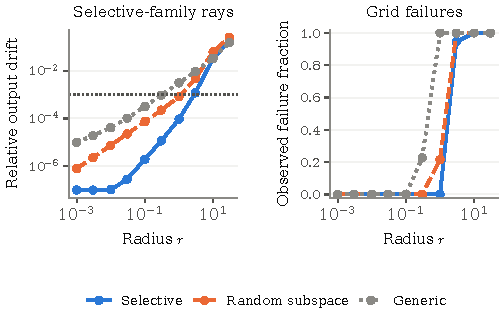
\includegraphics[width=3.024in]{resnet_common_rays.pdf}
\caption{ResNet selective-family rays, shown in the same format as the ViT study. Left: median relative RMS drift over 256 directions. Right: fraction exceeding $10^{-3}$ at any tested radius so far. Seed 0; no seed-variation band.}
\label{fig:resnet-common-rays}\label{tab:resnet-radii}
\end{figure}
